\documentclass{article} 
\usepackage[utf8]{inputenc}
\usepackage[margin=2.5cm]{geometry} % decrease the margin size

\usepackage{hyperref} % to include weblinks

\usepackage{graphicx} % handle images and figures
\usepackage{placeins} % to control placement of figures

\usepackage{amsmath} % general package for writing math
\usepackage{amsfonts} % math fonts for obscure symbols

\usepackage[nottoc]{tocbibind}
\usepackage[backend=biber,dateabbrev=false]{biblatex} % package for handling references
\addbibresource{references.bib}
\usepackage{csquotes}

\setlength{\parindent}{0pt} % remove indentation at the beginning of pargraphs

\begin{document}

\begin{titlepage}
    \begin{center}
        \vspace*{1cm}
        \Huge
        \textbf{Dynamic light scattering}
        
        \vspace{0.5cm}
        \LARGE
        Physikalisches Praktikum für Fortgeschrittene I
        
        \vspace{1.5cm}
        \textbf{Louis-Hendrik Barboutie and Rajon Bhuyan} \newline
        \textbf{7016306 \& 7029677}
        
        \vspace{0.5cm}
        \Large 
        Supervisor:
        
        \vfill

        \includegraphics[width=0.4\textwidth]{logo_uni.png}
        
        \Large
        9$^{\underline{\text{th}}}$ November 2022
    \end{center}
\end{titlepage}

% this is not strictly necessary and may be more clutter than useful
\tableofcontents

\newpage

\section{Basics} % this is a section

\subsection{Text} % this is a subsection
Each new line is a paragraph. You can write as much content as you want in a paragraph. To write in boldface, use \textbf{this is bold text}, for italic use \textit{this is italic text}.

Skipping a line creates a new paragraph, like I just did.

\subsection{Math Mode}

\subsubsection{Formulae}
To enter math mode you have several options: There's inline math with dollar symbols: $\sum_{k=0}^\infty \frac{1}{k^2} = \frac{\pi^2}{6}$ or there is the equation environment:
\begin{equation}
    \sum_{k=0}^\infty \frac{1}{k^2} = \frac{\pi^2}{6}
\end{equation}

and just add a star if you don't want the number:

\begin{equation*}
    \sum_{k=0}^\infty \frac{1}{k^2} = \frac{\pi^2}{6}
\end{equation*}

This is also equivalent to using:
\[
    \sum_{k=0}^\infty \frac{1}{k^2} = \frac{\pi^2}{6}
\]

other useful environment is align, the symbol "\&" will be the one the formulae will align on.

\begin{align}
    y &= (x+1)(x-1) \\
    &= x^2 - 1
\end{align}

and another useful one is the cases environment, which needs to be in math mode:
\begin{equation}
    \begin{cases}
        x + y = 2 \\
        x - y = 4
    \end{cases}
\end{equation}

\subsubsection{Symbols}
You can write a lot of symbols, every Greek letter by typing out its name, and with an uppercase first letter for the uppercase version: Gamma is $\gamma, \Gamma$, Delta is $\delta, \Delta$ etc.

You can write other letters with math fonts in the following way $\mathbb{R}$ and $\mathcal{O}$

A great collection of all the symbols is in this pdf: \url{https://www.cmor-faculty.rice.edu/~heinken/latex/symbols.pdf}, the nice thing about the url's is you can click them !

\subsection{Tables}

Creating a table is as easy as doing this:

\begin{table}[!ht] % !ht specifies to place it right here in the text
    \centering
    \begin{tabular}{c|lr} % here you specify the columns (with alignment: left, center or right) and vertical lines
        Experimentators & Age & Place of Birth \\ \hline
        Louis           & 41  & France \\
        Rajon           & 57  & India
    \end{tabular}
    \caption{This is the caption}
    \label{tab:TableAboutSomething}
\end{table}

Labels can be used to make references later, for example, in table \ref{tab:TableAboutSomething} I wrote our names in the first column.

\subsection{Figures}

Inserting a figure or picture can be done with:

\begin{figure}[!ht]
    \centering
    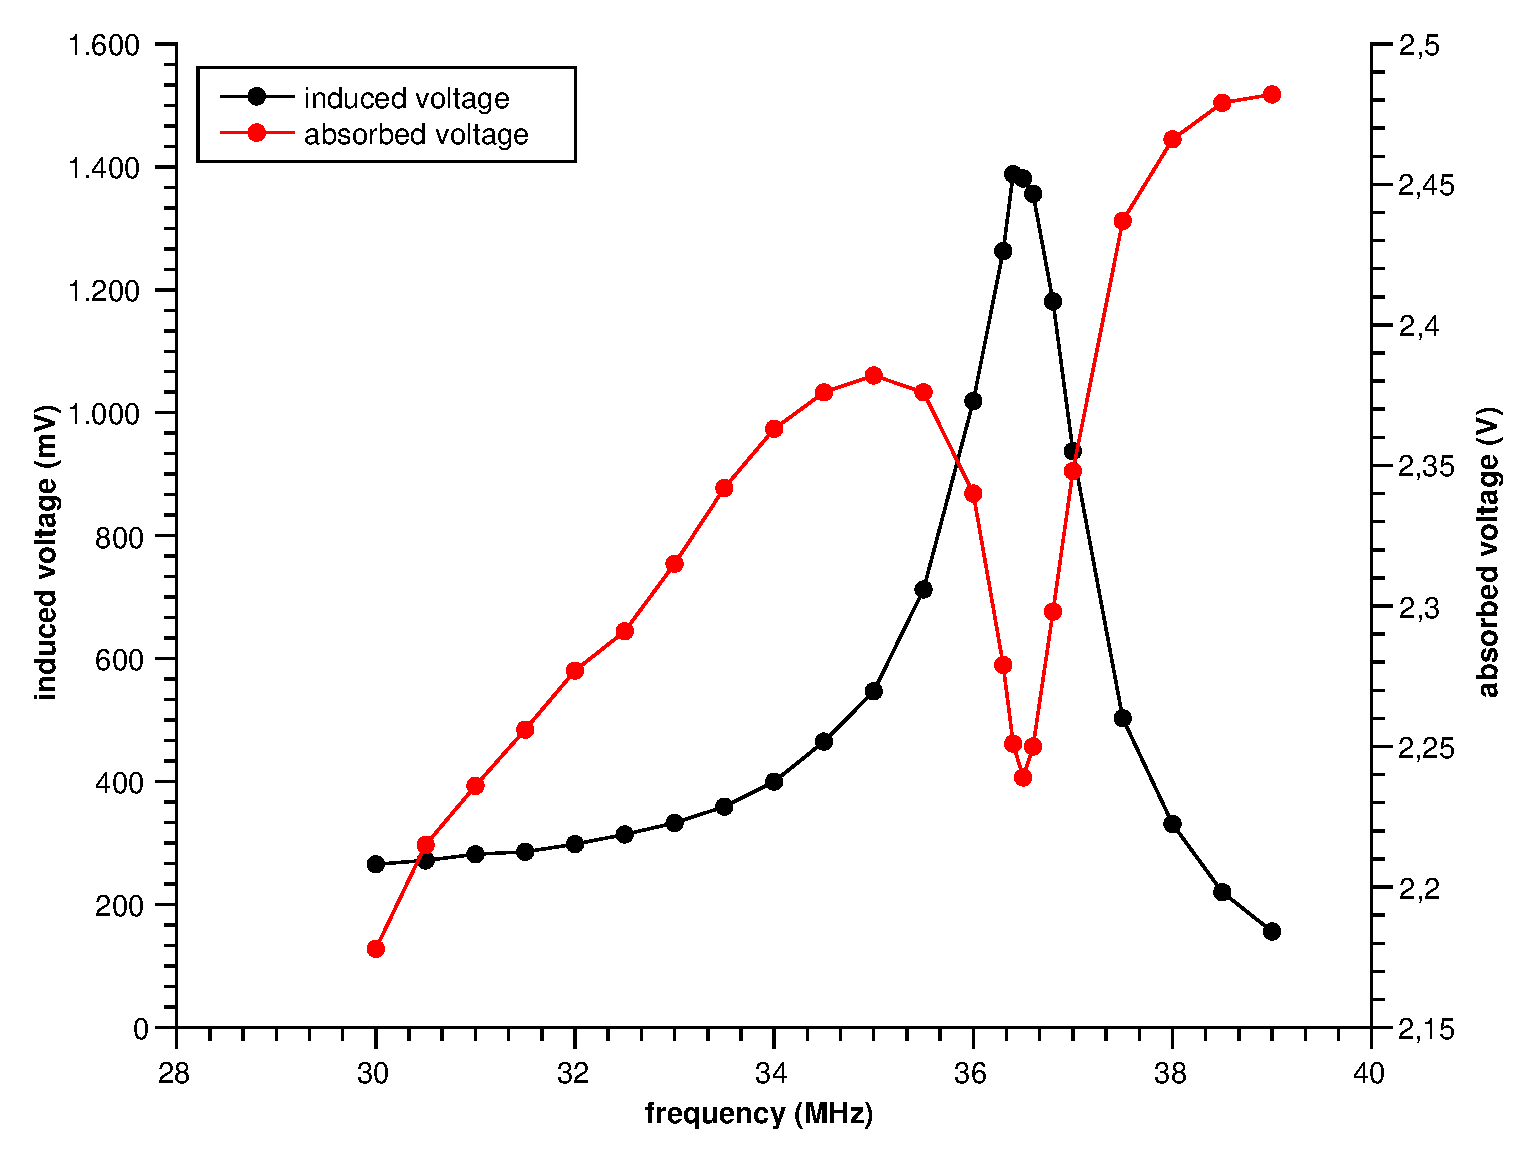
\includegraphics[width=0.7\textwidth,angle=0]{Capacitor1.eps}
    \caption{Graph of induced voltage as function of frequency}
    \label{fig:inducedV(frequency)}
\end{figure}
\FloatBarrier

You can control its size with the width modifier, its orientation with the angle modifier. The label works like for tables: figure \ref{fig:inducedV(frequency)} shows some data. Latex will take almost any obscure figure format you throw at it, here I fed it a .eps file, but it'll happily display .jpeg, .png, even .pdf. If the figure doesn't want to stay at the correct place, use the "floatbarrier" command, try to remove it from above and the picture will misbehave.

\section{Bibliography}

Writing the bibliography is a bit more complex, you need to first write the references using biblatex, and then cite them in the text for them to appear. For example, I could cite a paper with reference FluidFlow: \cite{FluidFlow}, or a book: \cite{KeelerNMR}. The nice thing about biblatex is the automatic formatting.

\printbibliography

\end{document}
